% Title page.
\title[Aula 05]{Oceanografia Física Descritiva}
\subtitle{Propriedades físicas da água do mar 02}
\author[Filipe Fernandes]{Filipe P. A. Fernandes}
\institute[unimonte]{Centro Universitário Monte Serrat}
\date[Setembro 2013]{27 de Setembro 2013}

\logo{
\includegraphics[scale=0.15]{../common/university_logo.png}}

\begin{document}

% The title page frame.
\begin{frame}[plain]
  \titlepage
\end{frame}

\section*{Outline}
\begin{frame}
\tableofcontents
\end{frame}

\section{Propriedades físicas da água do mar parte -- 02}

\begin{frame}
\frametitle{Perfis típicos -- Camadas}
    \begin{center}
        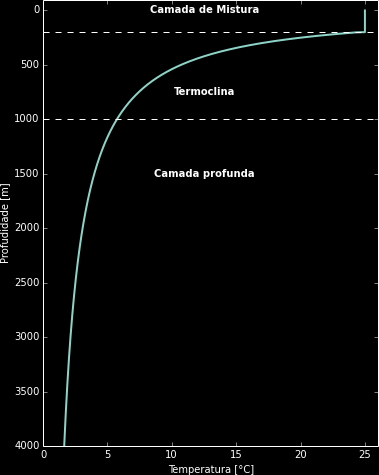
\includegraphics[scale=0.4]{./figures/temperature_profile.png}
    \end{center}
\end{frame}

\begin{frame}
\frametitle{Perfis típicos -- Variação latitudinal}
    \begin{center}
        \includegraphics[scale=0.25]{../figures/typical_profile_02.png}
    \end{center}
\end{frame}

\subsection{Equação de estado}
\begin{frame}
\frametitle{Densidade}
    \begin{block}{}
        Na prática medir densidade diretamente é muito complicado!
        A Solução é {\bf estimar} a densidade {\it in situ} usando a equação de estado.
    \end{block}
    \pause
    \begin{center}
        $\rho = \rho(T, S, p) = \frac{m}{V}\frac{\text{ [kg]}}{\text{ [m]}^3} $
    \end{center}
\end{frame}


\begin{frame}
\frametitle{Densidade}
    \begin{block}{Outra forma para densidade, o volume específico}
            $$\frac{1}{\rho} \equiv \alpha$$
            $$\alpha(T, S, p) = \frac{V}{m}\frac{\text{ [m]}^3}{\text{ [kg]}} $$
    \end{block}
\end{frame}


\begin{frame}
\frametitle{Linear EOS}
    \begin{block}{}
      Equação de estado linearizada (apenas para estimativas!)
      $\rho - \rho_o = -\alpha(T - T_o) + \beta(S - S_o) + \kappa p$,
    \end{block}
    \vspace{0.3cm}
    Onde:
    \pause
    $\rho_o = 1027 \frac{\text{kg}}{{\text{m}}^3}$,
    $T_o = 10$\textcelsius,
    $S = 35 \frac{\text{g}}{\text{kg}}$,
    $\alpha = 0.15 \frac{\text{kg}}{\text{m}^3\text{\textcelsius}}$,
    $\beta = 0.78 \frac{\text{kg}}{\text{m}^3\text{g/kg}}$,
    $\kappa = 4.5 \times 10^{-3} \frac{\text{kg}}{\text{m}^3\text{decibar}}$.
\end{frame}

\begin{frame}
\frametitle{Sumário EOS}
  \begin{itemize}[<+-| alert@+>]
    \item Em áreas costeiras a influência de $p$ pode ser ignorada;
    \item Áreas de alta carga de sedimentos em suspensão devemos incluir a
          massa de material seco;
    \item Os padrões de como calcular a Equação de estado são mantidos pela
          UNESCO;
  \end{itemize}
\end{frame}


\begin{frame}
\frametitle{Pressão hidrostática}
  O conhecimento do campo de densidade, portanto, é fundamental para o
  conhecimento do campo de pressão. A relação entre estes dois campos é a
  equação hidrostática:
    \begin{block}{Relembrando a pressão hidrostática.}
    $$\frac{\partial p}{\partial z} = g\rho$$
    \end{block}
    obs: Logo, podemos estimar a pressão nos oceanos usando o campo de
         densidade.
\end{frame}


\begin{frame}
\frametitle{Pressão hidrostática}
  \small{
  Para se chegar ao campo de pressão deve-se integrar verticalmente a equação
  anterior:
    \begin{block}{}
    $$h(z_1, z_2) = \int^{z_2}_{z_1}\delta(S, T, p)\rho_o dz$$
    \end{block}
    Denominamos $h$ de altura estérica ou se escrita em termos de pressão,
    altura dinâmica.
    \begin{block}{}
    $$D(p_1, p_2) = \int^{p_2}_{p_1}\delta(S, T, p)\rho_o dp$$
    \end{block}
    }
\end{frame}


\begin{frame}
\frametitle{Isopicnais e isóbaras}
    \begin{center}
        \includegraphics[scale=1]{../figures/isobars_isopycnals_01.png}
    \end{center}
\end{frame}


\begin{frame}
\frametitle{Isopicnais e isóbaras}
    \begin{center}
        \includegraphics[scale=1]{../figures/isobars_isopycnals_02.png}
    \end{center}
\end{frame}


\subsection{Propriedades conservativas vs. não conservativas}
\begin{frame}
\frametitle{Propriedades conservativas}
  \begin{itemize}[<+-| alert@+>]
    \item Abaixo da camada de superfície as propriedades como temperatura e
          salinidade somente podem ser alteradas por mistura ou advecção;
    \item Essas propriedades são ditas conservativas;
    \item Isto signifca que não há formação (origem), nem sourvedouro.
  \end{itemize}
    \pause
    \begin{block}{}
      $$\frac{\partial S}{\partial t} = \vec{v}\nabla{S}$$
    \end{block}
\end{frame}


\begin{frame}
\frametitle{Propriedades não conservativas}
  \begin{itemize}[<+-| alert@+>]
    \item Todas as outras propriedades como:
      \begin{enumerate}[<+-| alert@+>]
        \item Oxigênio;
        \item Nutrientes;
        \item {\bf Salinidade};
        \item {\bf Temperatura}.
      \end{enumerate}
      \item São afetadas por reações químicas ou processos biológicos.
      \item Essas propriedades são chamdas não conservativas!
  \end{itemize}
    \pause
    \begin{block}{}
      $$\frac{\partial S}{\partial t} = \vec{v}\nabla{S} + \Phi$$
    \end{block}
\end{frame}


\begin{frame}
\frametitle{Água tipo}
  \begin{itemize}[<+-| alert@+>]
    \item Como T-S podem ser considerados propriedades conservativas...
    \item ... Logo, abaixo da superfície, o par TS só muda por mistura e
          advecção.
    \item Assim, podemos identificar as massas d'água usando os pares de TS
          do seu local de formação.
    \item Esses pares são chamdas de água tipo.
  \end{itemize}
  \pause
    obs: Mas as massas de água podem assim ser identificadas apenas pelos seus pares temperatura-salinidade?
\end{frame}


\begin{frame}
\frametitle{Análise de massas d'água multiparamétrica}
  \begin{itemize}[<+-| alert@+>]
    \item Usando a razão de Redfiled (O:N:P $\equiv$ 138:15:1);
    \item Podemos estimar os nutrientes que não estão sendo reciclados;
    \item Assim, estimamos os nutrientes ``pré-formados'' que são ``quase-
          conservativos''!
    \item Esse é o princípio da AMO.  Enriquecendo os descritores de água tipo
          para além de T e S apenas.
  \end{itemize}
\end{frame}

\subsection{Gases dissolvidos}
\begin{frame}
\frametitle{Oxigênio dissolvido}
  \begin{itemize}[<+-| alert@+>]
    \item A solubilidade dos gases na água salgada é função da temperatura.
    \item Quanto mais baixa for a temperatura maior é solubilidade.
    \item A uma temperatura de 0\textcelsius{} um corpo de água com 35 g/kg de
          salinidade podeconter 8 ml de O$_2$ por litro.
    \item A uma temperatura de 20\textcelsius{} a quantidade de oxigênio
          dissolvido é de cerca de 5,4 ml/l.
  \end{itemize}
\end{frame}


\begin{frame}
\frametitle{Oxigênio dissolvido}
  \begin{itemize}[<+-| alert@+>]
    \item O oxigênio não se encontra naturalmente dissolvido de um modo
          uniforme no meio marinho.
    \item Habitualmente as maiores concentrações encontram-se nos primeiros
          10 a 20 m da coluna de água. Por quê?
    \item O teor em oxigênio dissolvido diminui sensivelmente com a
          profundidade. Os valores mínimos são atingidos entre 500--1000 m
    \item Abaixo desta zona o teor em oxigênio tende a aumentar. Novamente, por
          quê?
  \end{itemize}
\end{frame}


\begin{frame}
\frametitle{Oxigênio dissolvido}
  \begin{itemize}[<+-| alert@+>]
    \item Os valores mínimos são usualmente devidos à atividade biológica
          enquanto que o seu aumento abaixo desta zona deve ser associado ao
          influxo das águas mais frias quegeralmente são provenientes das
          regiões polares (ressurgência)
  \end{itemize}
\end{frame}


\begin{frame}
\frametitle{Perfil típico de gases dissolvidos}
    \begin{center}
        \includegraphics[scale=0.45]{../figures/oxigen.png}
    \end{center}
\end{frame}


\subsection{Estabilidade estática}
\begin{frame}
\frametitle{Estratificação de duas camadas}
\footnotesize{
  \begin{itemize}[<+-| alert@+>]
    \item O trabalho requerido para elevar uma parcela de água é:
          $\Delta PE = (\rho_2 - \rho_1)g\Delta z$;
    \item Densidade baixa sobre densidade alta = {\bf estável};
    \item Densidade aumentando com a profundidade = {\bf estável};
    \item Trabalho requer uma forma de energia;
    \pause
      \begin{enumerate}[<+-| alert@+>]
        \item Mecânica (Mistura)
        \item Térmica (Aquecimento/resfriamento)
      \end{enumerate}
    \item Se $\rho_1$ = $\rho_2$?
    \pause
      \begin{enumerate}[<+-| alert@+>]
        \item Não há trabalho para mover a parcela!
        \item Porque não há mudança na energia potencial.
      \end{enumerate}
    \item Na realidade a densidade no oceano cresce com a profundidade.
  \end{itemize}
  }
\end{frame}

\begin{frame}
\frametitle{Estratificação contínua.}
  \begin{block}{}
  Medida de estabilidade: $\text{E} = -\frac{1}{\rho}\frac{d\rho}{dz}$
  \end{block}
  \pause
  \begin{itemize}[<+-| alert@+>]
    \item E $>$ 0: Estável;
    \item E$_2$ $>$ E$_1$: E$_2$ é mais estável;
    \item E = 0: Estabilidade neutra;
    \item E $<$ 0: Instável (Convecção).
  \end{itemize}
\end{frame}

\begin{frame}
\frametitle{Estratificação contínua.}
  \begin{block}{}
  Frequência de estratificação: $N^2 = g\text{E} = -\frac{g}{\rho}\frac{d\rho}{dz}$
  \end{block}
  \pause
  \begin{itemize}[<+-| alert@+>]
    \item É a frequência natural de oscilação de uma parcela de água e $z$;
    \item $\rho$ é a densidade verdadeira e não a anomalia!
    \item Nos vamos revisitar isso no contexto de estabilidade dinâmica em
          breve...
  \end{itemize}
\end{frame}

\section{Dever de casa}
\begin{frame}
\frametitle{Dever de casa!}
    \begin{block}{}
        Estudar para a prova.
    \end{block}
    \vspace{0.3cm}
\end{frame}

\end{document}


